\subsection{HTTP request frames}

Voor deze test werd gebruik gemaakt van een sprite sheet met 15 frames op (figuur \ref{sheet}) en een animatie snelheid van 30 fps.

\begin{figure} [H]
	\centering
	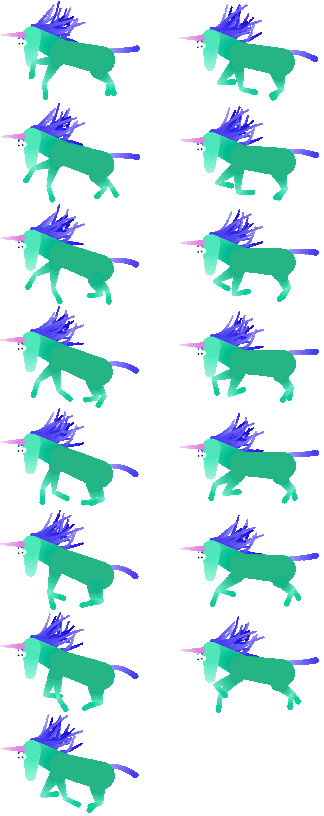
\includegraphics [scale=0.6] {img/charging.png}
	\caption{Sprite sheet met 15 frames (Figuur van \cite{stackoverflow})} \label{sheet}
\end{figure}

Bij de eerste test werdt de hele sprite sheet per frame ingeladen. Dit is om het effect te creëren dat de server elke frame genereert en doorstuurt naar de cliënt. Dit bleek zeer inefficiënt te zijn doordat de tijd om de frame op te halen met ethernet rond de 140 ms en met draadloos internet rond de 250 ms ligt (figuur \ref{draadloos} en figuur \ref{ethernet}).

\begin{figure} [H]
	\centering
	\begin{subfigure} [b] {0.45\textwidth}
		\centering
		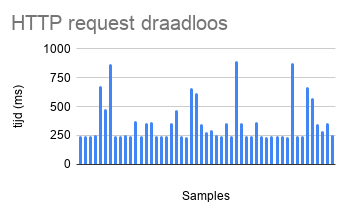
\includegraphics [width=\textwidth] {img/draadloos.png}
		\caption{HTTP request met draadloze verbinding} \label{draadloos}
	\end{subfigure}
	\begin{subfigure} [b] {0.45\textwidth}
		\centering
		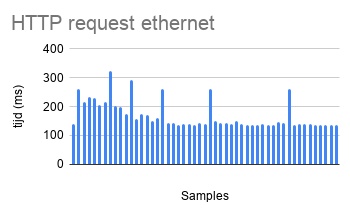
\includegraphics [width=\textwidth] {img/ethernet.png}
		\caption{HTTP request met ethernet verbinding} \label{ethernet}
	\end{subfigure}
\end{figure}

Hoewel de frames asynchroon worden ingeladen (figuur \ref{inladen}) is de animatie alles behalve ideaal. Door lange wachttijden zijn er veel frame skips en door de vele http requests wordt de verbinding gereset om de server niet te overbelasten met 30 requests per seconde (figuur \ref{reset}).

\begin{figure} [H]
	\centering
	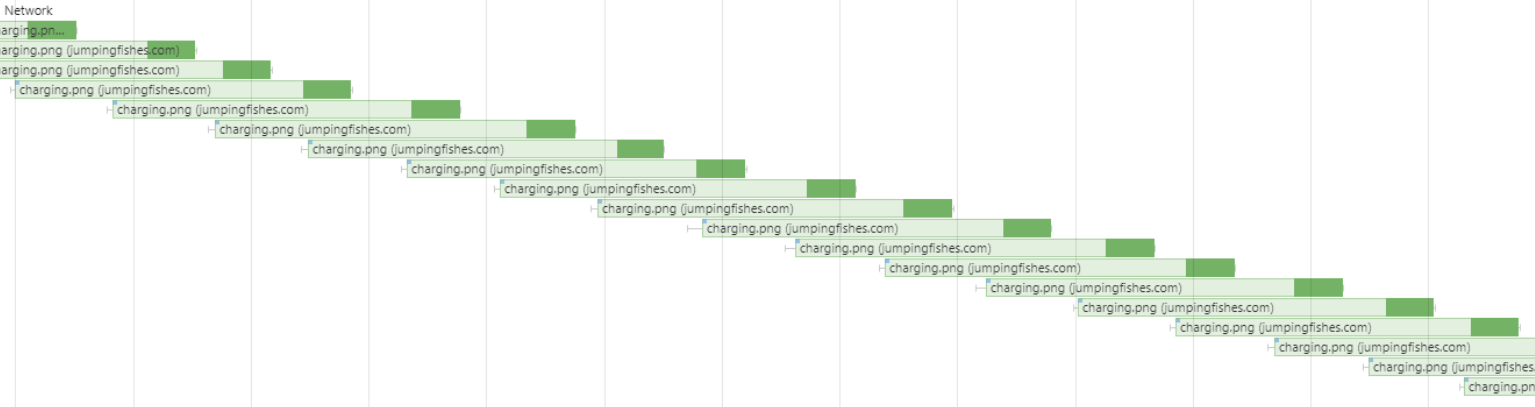
\includegraphics [scale=0.3] {img/inladen.png}
	\caption{Inladen van elke frame} \label{inladen}
\end{figure}

\begin{figure} [H]
	\centering
	
\includegraphics [scale=0.7] {img/reset.png}
	\caption{Connection reset door teveel requests} \label{reset}
\end{figure}

Bij de tweede test werd gebruik gemaakt van een buffer. De sprite sheet werd om de 0.5 seconden ingeladen zodat elke frame tijd had om te displayen ($30 \frac{frames}{sec} \frac{1}{15 frames}=\frac{0.5}{sec} $). Dit creëert het effect dat de server 15 frames genereert en doorstuurt in 1 keer i.p.v. frame per frame. Dit is duidelijk een verbetering want de server krijgt 15 keer minder requests (figuur \ref{inladen2}) en er zijn geen frame skips meer. Na het inladen van de sheet zal de cliënt de 15 frames achter elkaar drawen zonder te hoeven wachten op de server. Daarna zal de volgende sheet (of buffer) gebruikt worden.

\begin{figure} [H]
	\centering
	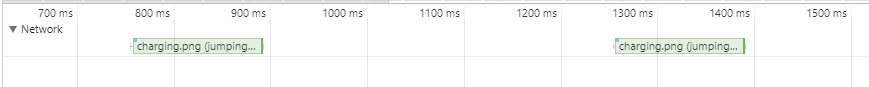
\includegraphics [scale=0.7] {img/inladen2.png}
	\caption{Inladen van de buffer} \label{inladen2}
\end{figure}